\section{Simulations}

Our experiments perform feedback alignment algorithm on both synthetic and real-world data with different regularization schemes. In particular, we compare the regularized feedback alignment (\cref{algo:fa-reg}) with its non-regularized counterpart (\cref{algo:fa}) on linear two-layer networks as well as the non-linear ones with different activation functions. We also evaluate the regularized feedback alignment algorithm with two-layer classification networks on \texttt{MNIST} dataset.

\paragraph{Synthetic data.}

For linear two-layer networks, we generate

\begin{figure}[h]
\centering

\begin{subfigure}[b]{.49\textwidth}
  \centering
  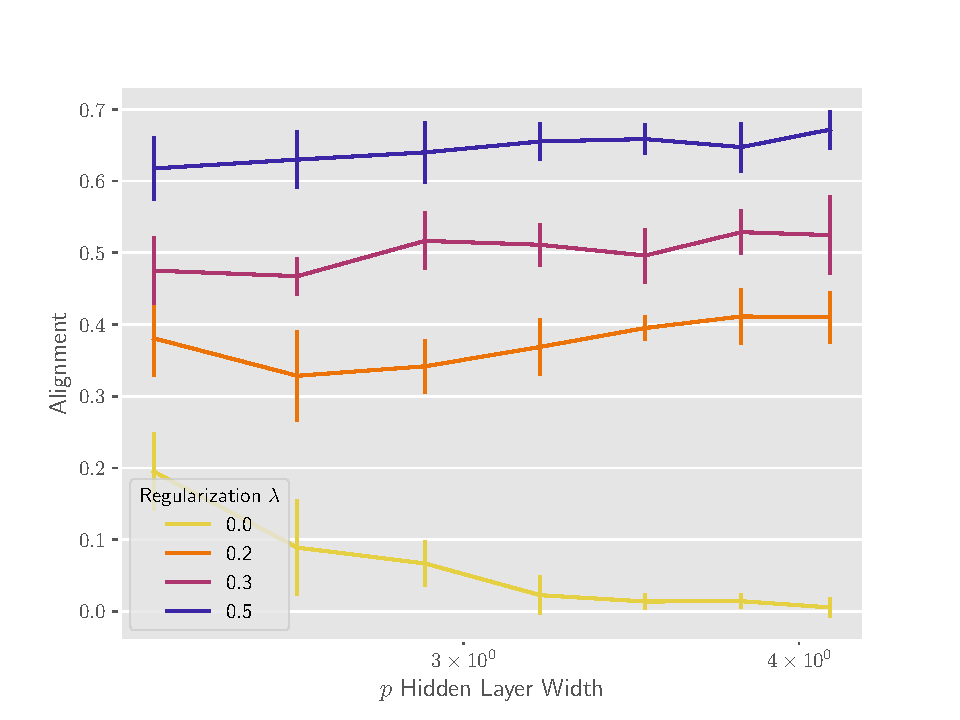
\includegraphics[width=\linewidth]{figures/align_lr_non_autograd_l2_v3.pdf}
  \caption{Alignment of linear network on linear regression data.}
  \label{fig:align_lr_non_autograd_l2}
\end{subfigure}\hfill
\begin{subfigure}[b]{.49\textwidth}
  \centering
  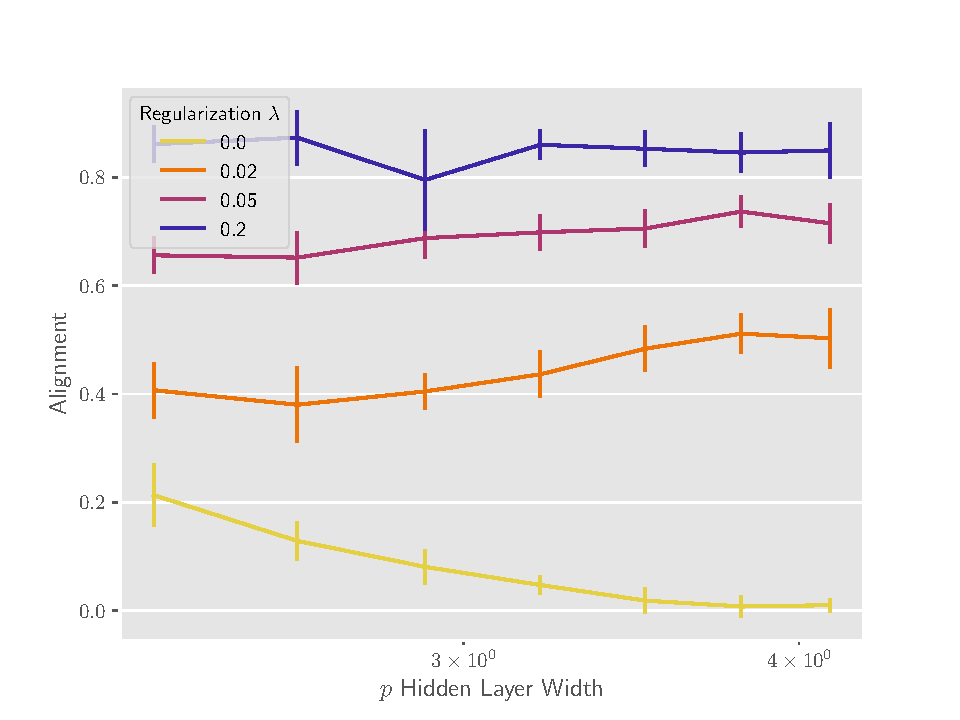
\includegraphics[width=\linewidth]{figures/align_nn_relu_autograd_l2_v4.pdf}
  \caption{Alignment of ReLU network on ReLU data.}
  \label{fig:align_nn_relu_autograd_l2}
\end{subfigure}

\medskip

\begin{subfigure}[b]{.49\textwidth}
  \centering
  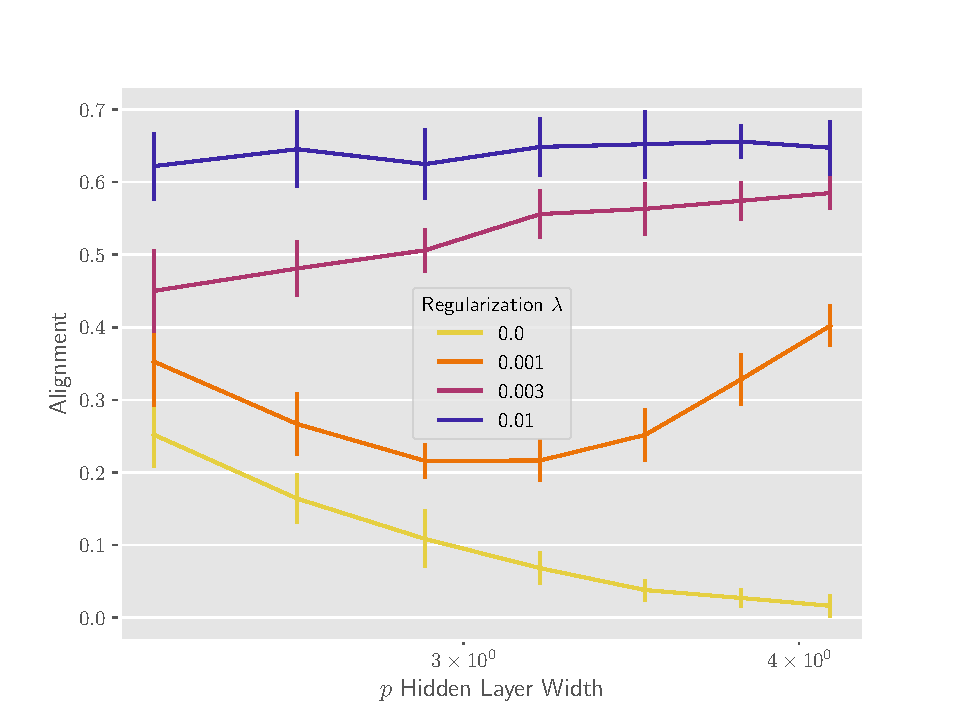
\includegraphics[width=\linewidth]{figures/align_nn_sigmoid_autograd_l2_v3.pdf}
  \caption{Alignment of Sigmoid network on Sigmoid data.}
  \label{fig:align_nn_sigmoid_autograd_l2}
\end{subfigure}\hfill
\begin{subfigure}[b]{.49\textwidth}
  \centering
  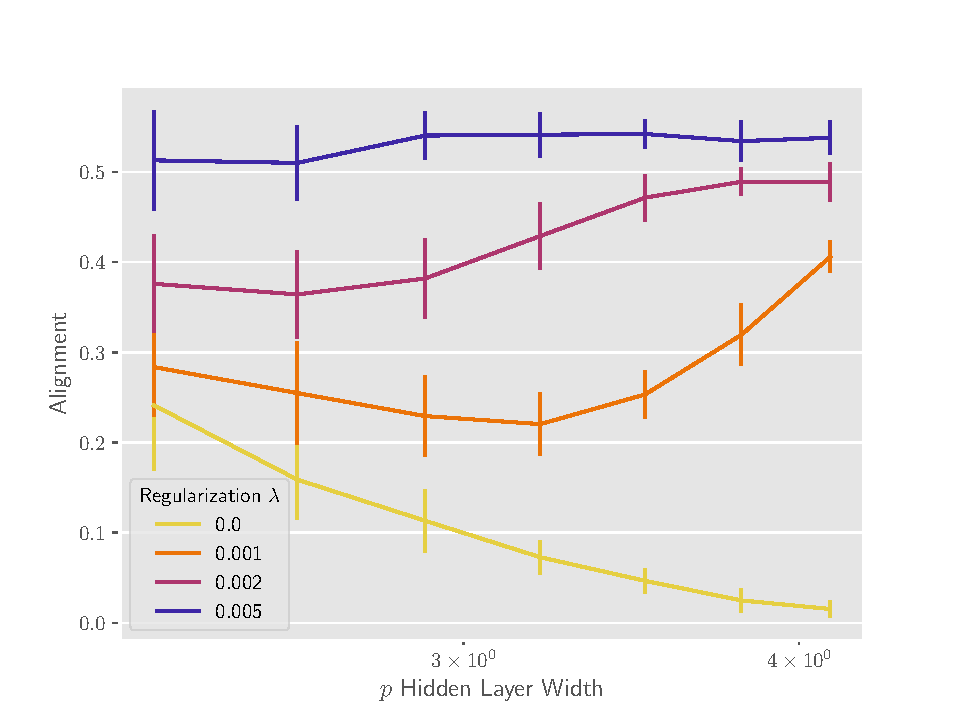
\includegraphics[width=\linewidth]{figures/align_nn_tanh_autograd_l2_v3.pdf}
  \caption{Alignment of Tanh network on Tanh data.}
  \label{fig:align_nn_tanh_autograd_l2}
\end{subfigure}
\caption{Synthetic data, l2. }
\label{fig:synthetic-l2}
\end{figure}

\begin{figure}[h]
\centering

\begin{subfigure}[b]{.49\textwidth}
  \centering
  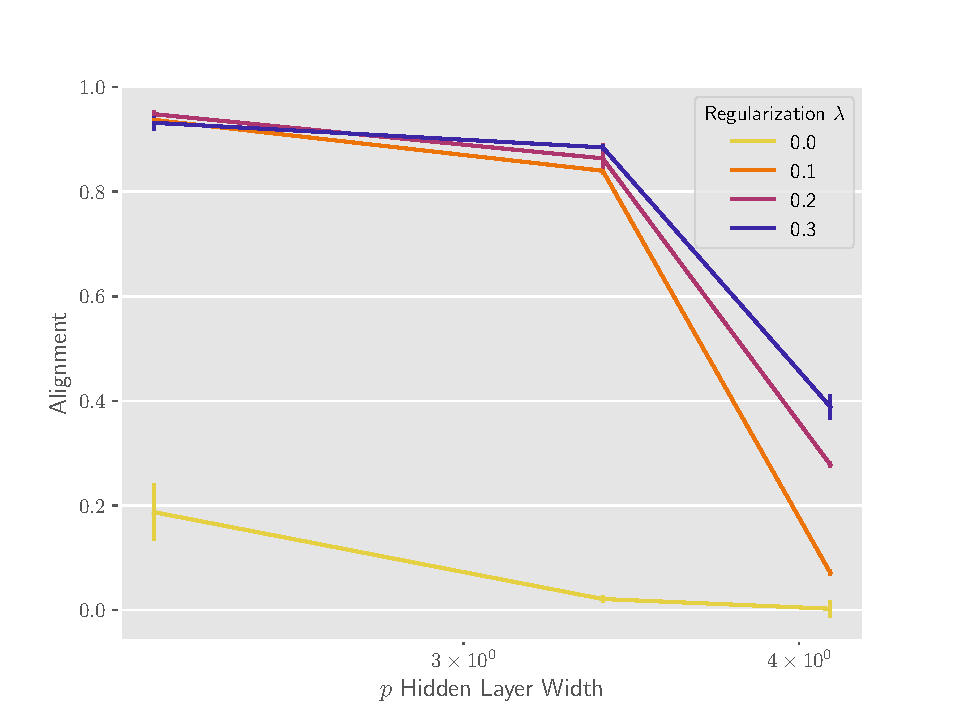
\includegraphics[width=\linewidth]{figures/align_lr_non_autograd_dropout_v2.pdf}
  \caption{Alignment of linear network with dropout on linear regression data.}
  \label{fig:align_lr_non_autograd_dropout}
\end{subfigure}\hfill
\begin{subfigure}[b]{.49\textwidth}
  \centering
  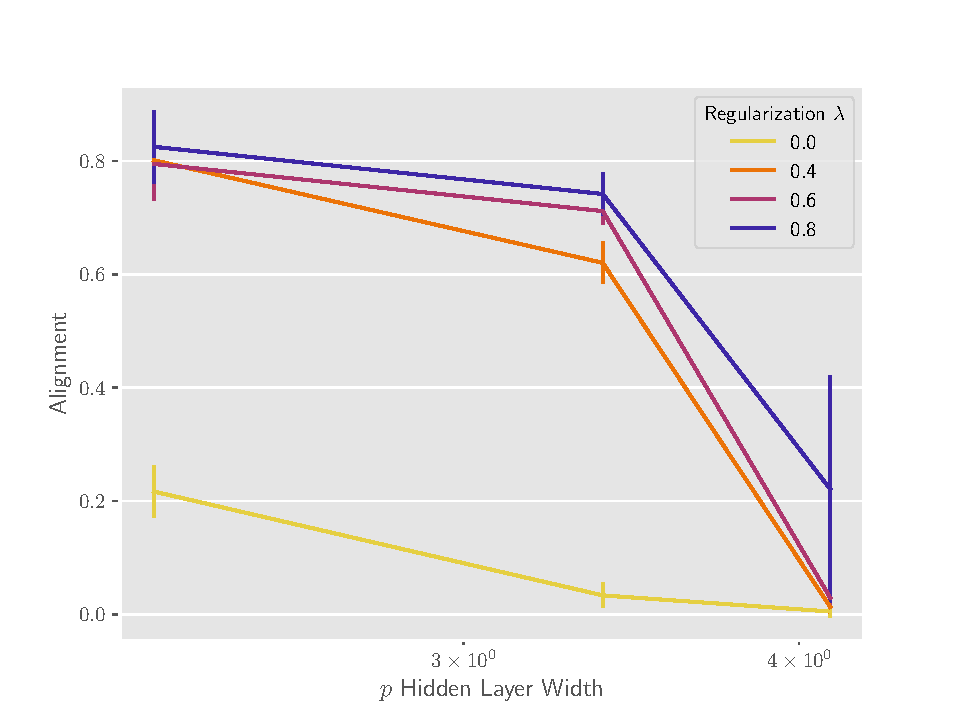
\includegraphics[width=\linewidth]{figures/align_nn_relu_autograd_dropout_v2.pdf}
  \caption{Alignment of ReLU network with dropout on ReLU data.}
  \label{fig:align_nn_relu_autograd_dropout}
\end{subfigure}

\medskip

\begin{subfigure}[b]{.49\textwidth}
  \centering
  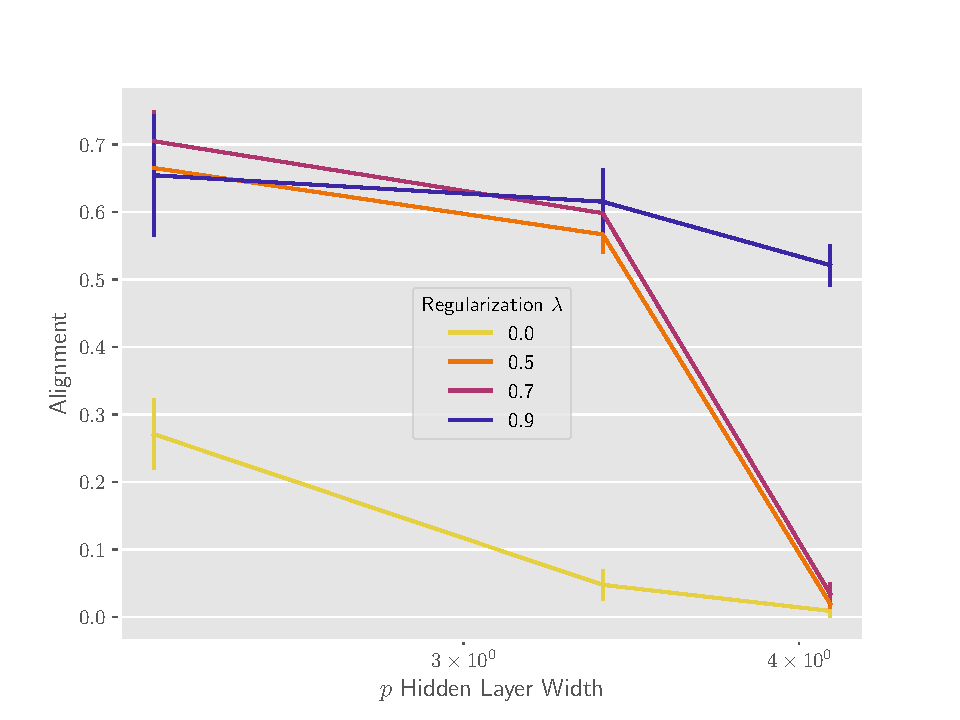
\includegraphics[width=\linewidth]{figures/align_nn_sigmoid_autograd_dropout_v2.pdf}
  \caption{Alignment of Sigmoid network with dropout on Sigmoid data.}
  \label{fig:align_nn_sigmoid_autograd_dropout}
\end{subfigure}\hfill
\begin{subfigure}[b]{.49\textwidth}
  \centering
  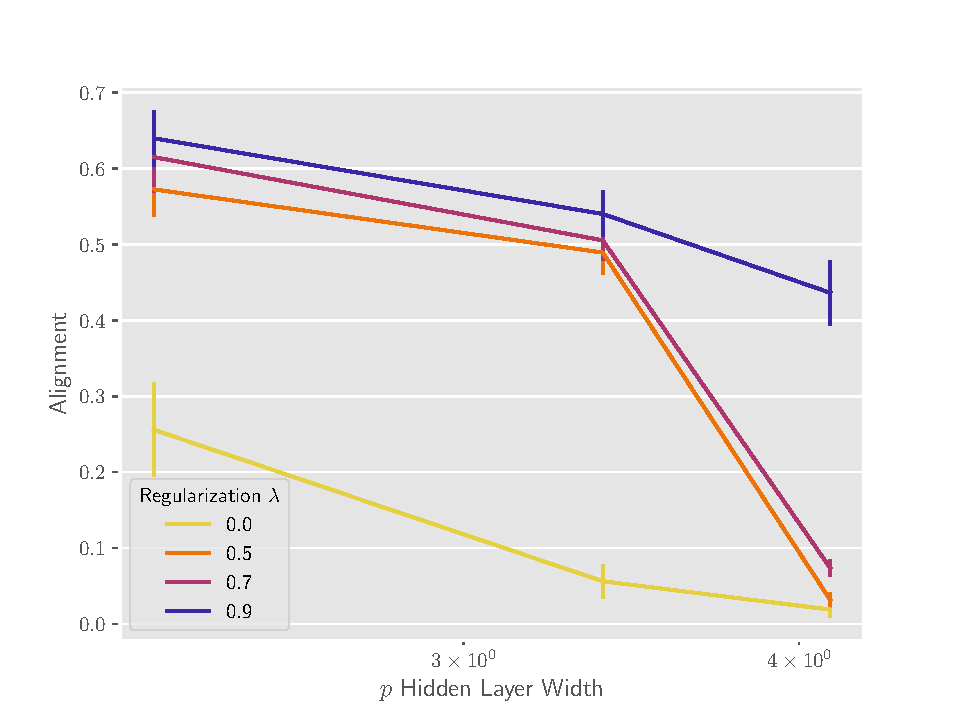
\includegraphics[width=\linewidth]{figures/align_nn_tanh_autograd_dropout_v2.pdf}
  \caption{Alignment of Tanh network with dropout on Tanh data.}
  \label{fig:align_nn_tanh_autograd_dropout}
\end{subfigure}
\caption{Synthetic data, dropout. }
\label{fig:synthetic-dropout}
\end{figure}

\paragraph{MNIST data.}